\documentclass[a4paper,11pt]{article}
\usepackage[T1]{fontenc}
\usepackage[utf8]{inputenc}
\usepackage{lmodern}
\input GetPackages

\title{MICE Target Simulation}
\author{Tom Lord, Paolo Franchini}

\begin{document}

\maketitle
\tableofcontents

\begin{abstract}
Simulation of the pion production coming out from the MICE target using the MARS simulation software and implementation of this simulation into the MICE Monte Carlo software.
\end{abstract}

\section{Motivation}

Non trivial discrepancies in the data versus Monte Carlo comparison have justified the necessity to reconsider the pions momentum distribution used as primary input of the MICE Monte Carlo.
The former model consisted in a fit done with three Gaussian of a pion distribution produced in 2008 with a earlier version of the MARS simulation software. Lack of documentation on this first study made hard to evaluate the goodness of the model. 

\section{The MICE target in the ISIS proton beam}

Brief description of the MICE target.

ISIS proton beam: energy, dimension, position...

\section{MARS simulation}

The design of the MICE target, in particular the surrounding structure, is defined as in~Fig.~\ref{fig:MARS1}. The presented design has been based on schematics (ref) and surveys (ref). The MICE beamline is orientated at 25 deg with respect to the ISIS beamline section where the target is located.

\begin{figure}
  \begin{center}
    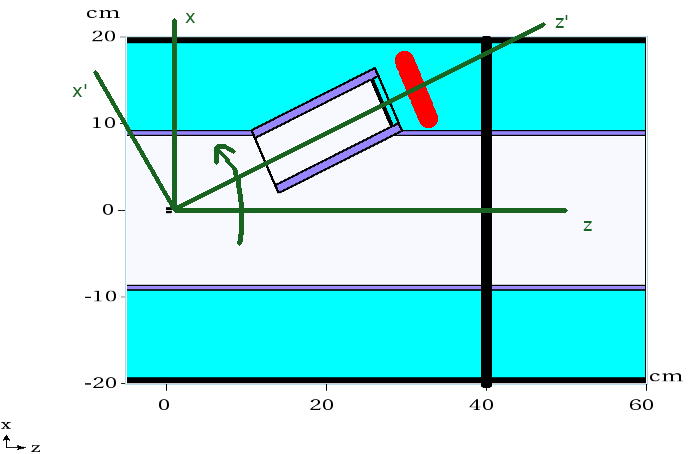
\includegraphics[width=1.0\columnwidth]{./figures/MARS1.png}
    \caption{Design of the target in the MARS simulation. TO BE CHANGED WITH SOMETHING NOT TOUCHED WITH PAINT. PLEASE SAME X-Y SCALES}
    \label{fig:MARS1}
  \end{center}
\end{figure}

\section{MAUS simulation}

The Monte Carlo in MICE is produced in a two-steps process. In the first step a pion beam in produced according to an initial momentum distribution and propagated using G4BL up to XXX where MAUS takes over propagating the particles through the remaining part of the beam line up to the EMR, passing for the cooling channel, according to the geometry and run selected to be simulated.

\subsection{Monte Carlo and data comparison}

Few figure of merits have been considered: time of flight of the particles between TOF0 and TOF1 and momentum distribution of pions and muons in the upstream tracker at station 5.
Simulations have been produced for 140, 200 and 240 MeV/c nominal pionic beams.

\section{Conclusions}

\begin{thebibliography}{9}
\bibitem{mars} https://mars.fnal.gov/
\bibitem{micenote1} MICE note #1, http://mice.iit.edu/micenotes/public/pdf/MICE0396/MICE0396.pdf
\bibitem{micenote2} MICE note #2, http://mice.iit.edu/micenotes/public/pdf/MICE0396/MICE0396.pdf
\end{thebibliography}


\end{document}
